\providecommand{\master}{..}
\documentclass[../Master.tex]{subfiles}
\begin{document}

\begin{figure}
    \centering
    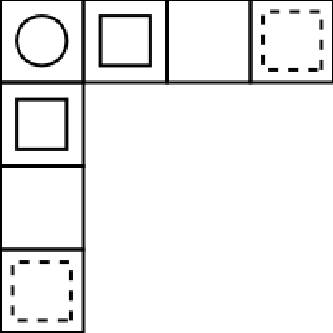
\includegraphics[scale=0.7]{\master/Graphics/soko1}
    \caption{\label{fig:simpleSokoban} A simple sokoban world. The circle is the sokoban, the squares are crates, and the dashed lines denote goal tiles.}
\end{figure}

We will now present a formalization of the sokoban world introduced in section \ref{sec:Algorithm} based on the PDDL specification presented in \cite{BS2011}.

\subsubsection{Problem specification}
Any given sokoban problem, such as the one illustrated in figure \ref{fig:simpleSokoban}, contains a number of $crate$ objects (denoted $c_1, \dots, c_n$) as well as a number of $tile$ objects (denoted $t_1, \dots, t_k$). To describe how the tiles are interconnected, we introduce the predicates $hAdj(t_1,t_2)$ and $vAdj(t_1,t_3)$, respectively denoting that tile $t_1$ is horizontally adjacent to tile $t_2$ and vertically adjacent to $t_3$. It is clear that these relations are symmetric; if $t_i$ is vertically adjacent to $t_j$, then $t_j$ is also vertically adjacent to $t_i$ (similarly for horizontal adjacency). In the framework presented above, there is no machinery for aximoatic reasoning, hence this symmetry must be manually encoded by the problem designer by --- in the above example --- adding the predicates $hAdj(t_2,t_1)$ and $vAdj(t_3,t_1)$.

Locations of the crates can be encoded with the predicate $at(c, t)$, denoting that crate $c$ is on tile $t$. Locations of goal tiles and the sokoban are represented with the predicates $goal(t)$ and $sokobanAt(t)$, respectively.

The initial state of a problem can now be represented by a conjunction of the these predicates. The state illustrated in figure \ref{fig:simpleSokoban} can be encoded by the formula in \eqref{eq:simpleSokoSpec}. The \textit{goal} of any sokoban problem is that each crate is positioned at a goal tile, denoted by the conjunction $atGoal(c_1) \land atGoal(c_2) \land \cdots \land atGoal(c_n)$.

\begin{gather}
\begin{gathered} \label{eq:simpleSokoSpec}
    hAdj(t_1, t_2) \land hAdj(t_2, t_3) \land hAdj(t_3, t_4) \land \\
    hAdj(t_2, t_1) \land hAdj(t_3, t_2) \land hAdj(t_4, t_3) \land \\
    vAdj(t_1, t_5) \land vAdj(t_5, t_6) \land \\
    vAdj(t_5, t_1) \land vAdj(t_6, t_5) \land \\
    goal(t_4) \land goal(t_6) \land \\
    sokobanAt(t_1) \land at(c_1, t_2) \land at(c_2, t_5) \land \\
    clear(t_3) \land clear(t_4) \land clear(t_6)
\end{gathered}
\end{gather}


\graphicspath{{.../Graphics/}}

\subsubsection*{Domain specification}
When designing a virtual or physical robot capable of solving a sokoban puzzle, it would be sufficient to equip it with a $move$ action which, given a direction or an adjacent tile, would relocate the sokoban appropriately, displacing any crates in the way. However, as STRIPS-style action schemas can only contain a single effect, it does not allow an action to, for example, push a crate \textit{if}  it is on the tile the sokoban is moving to. Instead, this requires different actions, which are outlined below:

The effect of a movement action from tile $t_1$ to tile $t_2$ is that the sokoban is no longer present at $t_1$, but appears on $t_2$. Since there are no notion of variables in STRIPS-style action specifications, both $t_1$ and $t_2$ are given as arguments to the action, so that it can be asserted whether the sokoban is actually located at $t_1$ and whether it is possible to relocate it to $t_2$. Since pushing a crate has a different effect, and must therefore be implemented as another action, the destination tile must be empty for the movement action to succeed. Since STRIPS-style action schemas do not allow existentially or universally quantified formulae, the $at$ predicate can not be used, and the $clear$ predicate is used instead.

As per the sokoban rules, movement from $t_1$ to $t_2$ is allowed only if the two tiles are either horizontally \textit{or} vertically adjacent. As preconditions can not contain disjunctions, and there can only be one precondition per action schema, two schemas are required for movement: One (\textit{move-h}) containing the precondition $hAdj(t_1,t_2)$ and the other (\textit{move-v}) the precondition $vAdj(t_1, t_2)$.
In \eqref{act:moveh} the \textit{move-h} action is listed. The \textit{move-v} action is similar, except for having $vAdj$ as a precondition instead of $hAdj$.

\begin{align}
\begin{split} \label{act:moveh}
\textsc{Action} &\; \textit{move-h}(from, to): \\
\textsc{Pre}: \; & sokobanAt(from) \land hAdj(from, to) \land clear(to) \\
\textsc{Eff}: \; & \neg sokobanAt(from) \land sokobanAt(to) \land \\
& clear(from) \land clear(to)
\end{split}
\end{align}

The action schema for pushing a crate depends on four parameters: the crate to push, its location, the location, its destination, and the location of the sokoban. As for the movement actions, two different push actions are required; one for pushing horizontally (depicted in \eqref{act:pushh}) and one for pushing vertically. Its preconditions assert that the sokoban is horizontally adjacent to the crate, and that the crate is horizontally adjacent to the destination. It also ensures that the destination is an empty tile, which precludes it from being the tile inhabited by the sokoban, ensuring that the sokoban can not just swap places with the crate, which is not allowed.

As the effect of moving a crate to a goal tile is different from that of moving it onto a non-goal tile, the former requires its own \textit{push-h-goal}  and \textit{push-v-goal} actions (listed in \eqref{act:pushhgoal}). Hence, the destination tile is required to be a non-goal tile for the push action, and the effect is that the crate is not occupying a goal tile.

\begin{align}
\begin{split} \label{act:pushh}
\textsc{Action} &\; \textit{push-h}(crate, sokoban, from, to): \\
\textsc{Pre}: \; & sokobanAt(sokoban) \land
at(crate, from) \land
\neg goal(to) \land \\
& hAdj(sokoban, from) \land
hAdj(from, to) \land
clear(to)
\\
\textsc{Eff}: \; & \neg sokobanAt(sokoban) \land
sokobanAt(from) \land
clear(sokoban) \land \\
& \neg at(crate, from) \land
at(crate, to) \land
\neg clear(to) \land
\neg atGoal(crate)
\end{split}
\end{align}

\begin{align}
\begin{split} \label{act:pushhgoal}
\textsc{Action} &\; \textit{push-h-goal}(crate, sokoban, from, to): \\
\textsc{Pre}: \; & sokobanAt(sokoban) \land
at(crate, from) \land
goal(to) \land \\
& hAdj(sokoban, from) \land
hAdj(from, to) \land
clear(to) \land
\\
\textsc{Eff}: \; & \neg sokobanAt(sokoban) \land
sokobanAt(from) \land
clear(sokoban) \land \\
& \neg at(crate, from) \land
at(crate, to) \land
\neg clear(to) \land
atGoal(crate)
\end{split}
\end{align}

In total, six different action schemas are required for the sokoban domain, and more would be required if the domain was to be made reversible.

\section{Conditional Sokoban action schemas}

We will now present a formalization of the Sokoban domain using conditional effects. We will adhere to the restrictions given in Chapter~\ref{chp:ca}, the most important of which are ``No action parameters'' and ``No disjuntive preconditions''. Additionally, the action schemas contain no preconditions, and their effects consists solely of conjunctions of conditionals.

Initially, observe that the domain and problem specifications can not readily be reused under these restrictions. For example, the adjacency relations carry no information about direction, i.e.\ whether one tile is to the left or right of another, but only that they are adjacent. This poses a problem when effects can only be described in terms of universally quantified predicates, as this could for example make the sokoban move to two horizontally adjacent, unoccupied tiles at once.

Instead, we

\begin{align*}
\actact & \textit{move-west(): } &  \\
& \forall x, y
    \left[
        \begin{gathered}
            sokobanAt(x) \land 
            \\ \neg sokobanAt(y) 
        \end{gathered}
    \right]
    \quad when \quad
    \left[ 
        \begin{gathered}
            sokobanAt(y) \land hAdj(x,y) \\ 
            \land \neg boxAt(x)
        \end{gathered}
    \right]
\end{align*}

\begin{align*}
    \actact & \textit{push-west(): } & \\
    & \forall x, y, z
    \left[ 
        \begin{gathered}
            \neg goalSolved(y) \\
            \land at(x) \land \neg at (y) \\
            \land sokobanAt(y) \\
            \land \neg sokobanAt(z) 
        \end{gathered}
    \right]
    \quad when \quad
    \left[
        \begin{gathered}
            at(y) \land \neg at(x) \\
            \land sokobanAt(z) \\ 
            \land hAdj (y,z) \land hAdj (x,y) \\
            \land \neg at(x)
        \end{gathered}
    \right] \\
    & \land \\
    & \forall x, y, z
    \left[
        goalSolved(x)
    \right]
    \quad when \quad
    \left[
        \begin{gathered}
            goal(x) \\
            \land at(y) \land \neg at(x) \\ 
            \land sokobanAt(z) \\ 
            \land hAdj (y,z) \land hAdj (x,y) \\
        \end{gathered}
    \right]
\end{align*}
% \begin{split}
%         \actact & move-west():
%         \forall x, y &\left[
%             \begin{split}
%                 hej & \\
%                 hej &
%             \end{split}
%             \right] \\
%         \end{split}
\end{document}
